\subsubsection{Convolutional layer} \label{subs:2dconv}
%
Fully-connected layer are non-linear classifiers, they take the extracted features of the input and converted as a one-dimension vector \cite{khan_survey_2020}. As a result, usually, the fully-connected layers are placed at the end of \acrshort{cnn}s, after that the first layers extract features from the input \cite{liu_fpga-based_2019}. The layers extracting features are the \textbf{convolutional layers}.

The main operation in a \acrshort{cnn} is the convolution which consists of extracting the features from the input image also called input \acrfull{fm} \cite{liu_fpga-based_2019, zhao_towards_2018}. It is the main operation on a \acrshort{cnn}, and it is the layer that gives the network its name. The first layer extracts low-level features of the input \acrshort{fm} while the deepest layers use these low-level features to build high-level ones \cite{goodfellow_deep_2016}.

\begin{figure}
    \centering
    %
    \begin{subfigure}{.32\textwidth}
    \centering
    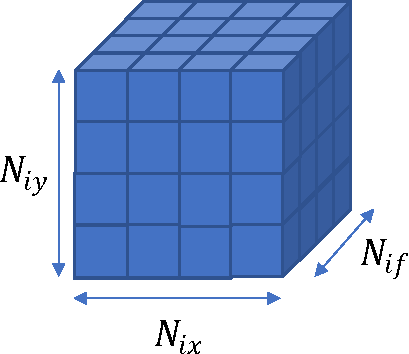
\includegraphics[width=\linewidth]{notifm.pdf}
    \caption{Input \acrshort{fm}}
    \label{fig:notation:ifm}
    \end{subfigure}
    %
    \begin{subfigure}{.32\textwidth}
    \centering
    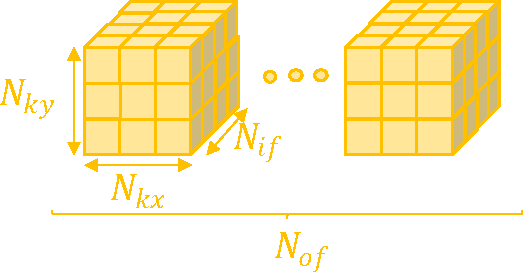
\includegraphics[width=\linewidth]{notk.pdf}
    \caption{A convolution kernel}
    \label{fig:notation:k}
    \end{subfigure}
    %
    \begin{subfigure}{.32\textwidth}
    \centering
    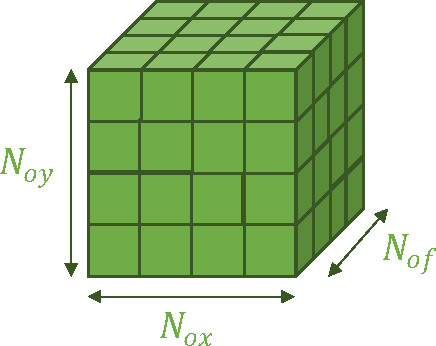
\includegraphics[width=\linewidth]{notofm.pdf}
    \caption{Output \acrshort{fm}}
    \label{fig:notation:ofm}
    \end{subfigure}
    %
    \caption{Volumes involved in the convolution operations}
    \label{fig:notconv}
\end{figure}
%
The notation for describing the different entities are inspired by \cite{ma_optimizing_2018}. The input \acrshort{fm} is characterized by 3 parameters: \textbf{$N_{ix}$} the width, \textbf{$N_{iy}$} the height, and \textbf{$N_{if}$} the depth. As shown on Figure \ref{fig:notation:ifm} this FM can be seen as successive layers of pixels forming a cuboid. Then, the convolution layer is used to correlate this FM and a 4D filter in order to build an output FM with high-level features \cite{zhao_towards_2018}.
This filter is composed of $N_{of}$ kernels, where each kernel has size $N_{kx} \times N_{ky} \times N_{if}$. and the output FM is also characterized by three parameters: its width $N_{ox}$, its height $N_{oy}$ and its depth $N_{of}$, as can be seen on Figure \ref{fig:notation:k} and \ref{fig:notation:ofm}, respectively.

\begin{figure}
    \centering
    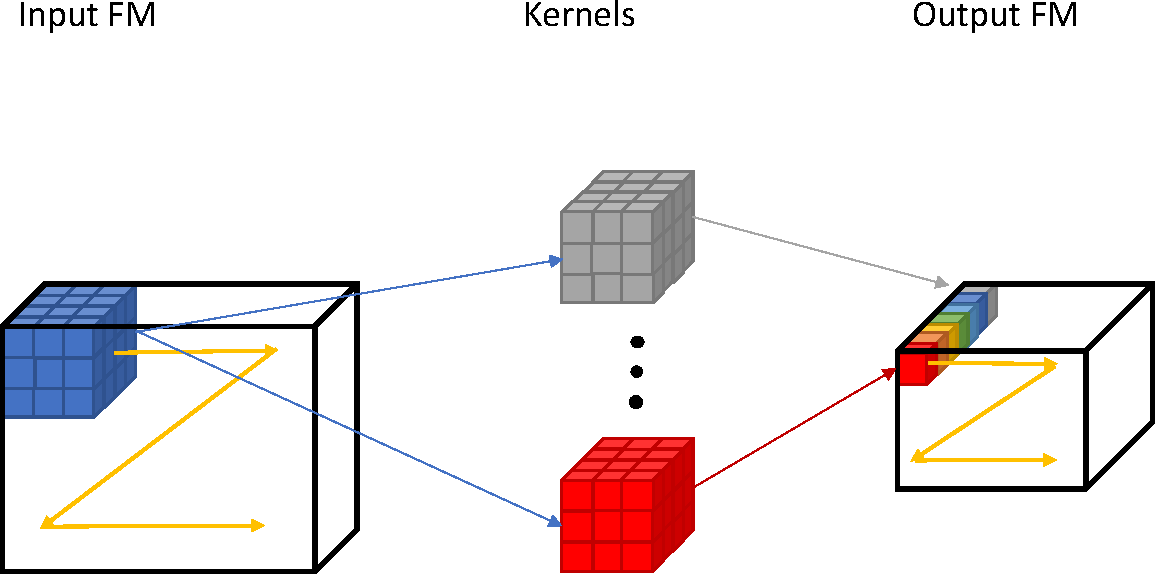
\includegraphics[width=\textwidth]{conv.pdf}
    \caption{Convolution operation}
    \label{fig:convolution}
\end{figure}
%
The convolution is a specialized linear operation which can be seen on Figure \ref{fig:convolution} and which is divided in three steps \cite{matteucci_artificial_2019, zhu_efficient_2020}:
%
\begin{enumerate}
    \item A window of the same size than the kernel extracts corresponding chunk of pixels from the input \acrshort{fm}.
    \item A multiplication of the chunk of pixels with the kernel is performed.
    \item The output pixels are summed up to produce one output pixel.
\end{enumerate}
%
Then, the kernel is shifted on the input FM and selects another chunk of pixels which is submitted to these convolutions steps, and so on until the whole input \acrshort{fm} has been convolutionned. This operation produces a channel of the output \acrshort{fm}, where the output pixel at position $(x, y)$ has been obtained by the movement of the sliding window from the top left of the input FM. In conclusion, one kernel generates one channel of output FM but there are actually $N_{of}$ kernels which produces then $N_{of}$ channels.

Except for $1 \times 1$ kernel, a spatial reduction between the input and output \acrshort{fm}s is observed, while there is an increase in the number of channels. It is explained by the fact that the sliding window movements can not go beyond the size of the input \acrshort{fm}. We can express the spatial reduction using equation \eqref{label:conv_spatial_red} \cite{ma_optimizing_2018}.
%
\begin{equation}
    N_{o\{x,y\}} = N_{i\{x,y\}} - N_{k\{x,y\}} + 1
    \label{label:conv_spatial_red}
\end{equation}
%
Therefore, \textit{padding} can be used on the boundaries in order avoid this spatial reduction. It consists of padding the edges with extra pixels (usually 0 value) \cite{liu_fpga-based_2019}.

The kernel can be shifted of different amount of pixels on the input FM which is called the \textit{stride} and is initially set to 1. If the stride is increased, the spatial dimensions of the output FM is decreased \cite{liu_fpga-based_2019}. For example, if a padding and a stride of 2 are used : $\frac{N_{ix}}{N_{ox}} = \frac{N_{iy}}{N_{oy}} = \frac{1}{2}$, and the output \acrshort{fm} has 4 times fewer pixels. Equation \eqref{label:conv_spatial_red_tot} represents the spatial reduction during convolution in function of the stride and the padding \cite{ma_optimizing_2018}. There are also other ways to introduce spatial reduction and one of them will be develope in Section \ref{subs:pooling}.
%
\begin{equation}
    N_{o\{x,y\}} = \left\lfloor \frac{ N_{i\{x,y\}}}{S} \right\rfloor - N_{k\{x,y\}} + 1
    \label{label:conv_spatial_red_tot}
\end{equation}

Finally, the whole convolution operation can be mathematically defined by Equation \eqref{eq:conv} \cite{abdelouahab_accelerating_2018}.
%
{\small
\begin{equation}
    \begin{split}
        \forall ox \in \{ 1, ..., N&_{ox} \}, oy \in \{ 1, ..., N_{oy} \}, of \in \{ 1, ..., N_{of} \}: \\
        FM_O[ox, oy, oc&] = \sum^{N_{if}}_{if=1}
        \sum^{N_{kx}}_{kx=1}
        \sum^{N_{ky}}_{ky=1}\\
        & FM_I \left[ ox \cdot S + kx - \left\lfloor \frac{N_{kx}}{2} \right\rfloor,  oy \cdot S + ky - \left\lfloor \frac{N_{ky}}{2} \right\rfloor, if \right] \cdot
        W^{of}_{if} \left[ kx, ky \right]
    \end{split}
    \label{eq:conv}
\end{equation}
}

According to \textcite{goodfellow_deep_2016}, the convolutional layer shows several advantages compared to the fully-connected layer. Indeed, the convolutional layer is sparsely connected, which means that there are fewer connections between the different layers. The convolutional layer is then easier to train and the convolution keeps spatial information. Moreover, it has also parameter sharing: the same kernel is used to compute one channel of the output \acrshort{fm} and fewer parameters are needed. To illustrate this weight reduction, in AlexNet \cite{krizhevsky_imagenet_2012}, 94\% of the weights are used in the fully-connected layers. But as said previously, convolution is a computationally heavy operation. For example, in VGG-11, 98.2\% of the operations are done in the convolution layers \cite{guo_survey_2018}. Furthermore, if the input \acrshort{fm} is a vector ($N_{ix} = N_{iy} = 1$), then it means that the convolution and the fully-connected layer perform the same operation.

As the convolution has a huge arithmetic complexity, we see in the following section \ref{subs:dsc} an alternate way to perform convolution while reducing its complexity.
